\documentclass[aspectratio=169,11pt]{beamer}
\usepackage[T1]{fontenc}
\usepackage{lmodern,amsmath,amssymb,mathtools,bm,booktabs,array,graphicx,tikz}
\usetikzlibrary{arrows.meta,positioning,calc,decorations.pathreplacing,patterns}
\definecolor{ink}{HTML}{17344D}\definecolor{accent}{HTML}{087E8B}\definecolor{pale}{HTML}{EDF5F5}\definecolor{gold}{HTML}{AD6B19}
\providecommand{\dd}{\,\mathrm{d}}\providecommand{\R}{\mathbb{R}}
\providecommand{\E}{\mathbb{E}}\providecommand{\Var}{\operatorname{Var}}
\providecommand{\Cov}{\operatorname{Cov}}\providecommand{\diag}{\operatorname{diag}}
\providecommand{\norm}[1]{\left\lVert#1\right\rVert}
\providecommand{\abs}[1]{\left|#1\right|}
\usefonttheme{professionalfonts}
\setbeamercolor{normal text}{fg=black,bg=white}
\setbeamercolor{frametitle}{fg=ink,bg=white}
\setbeamercolor{title}{fg=ink}\setbeamercolor{structure}{fg=accent}
\setbeamercolor{block title}{fg=ink,bg=pale}\setbeamercolor{block body}{fg=black,bg=pale!40}
\setbeamercolor{alerted text}{fg=accent}
\setbeamerfont{frametitle}{size=\Large,series=\bfseries}
\setbeamerfont{title}{size=\LARGE,series=\bfseries}
\setbeamertemplate{navigation symbols}{}
\setbeamersize{text margin left=.7cm,text margin right=.7cm}
\setbeamertemplate{frametitle}{\vspace{.18cm}\insertframetitle\par\vspace{.1cm}{\color{accent}\hrule height .6pt}\vspace{.12cm}}
\newcommand{\notestarget}{notes.pdf}\newcommand{\noteslabel}{Notes}
\setbeamertemplate{footline}{\hspace{.7cm}\color{ink}\scriptsize Scientific Computing in Python\quad\href{\notestarget}{\noteslabel}\hfill\insertframenumber\,/\,\inserttotalframenumber\hspace{.7cm}\vspace{.18cm}}
\setbeamercovered{invisible}
\hypersetup{pdfauthor={Zan Ahmad},pdftitle={Least squares, principal components, and clustering},pdfpagemode=UseNone}
\begin{document}
\begin{frame}[plain]\vfill
{\small\color{accent} Scientific Computing in Python \quad Lecture 5}\par\medskip
{\raggedright\hyphenpenalty=10000\exhyphenpenalty=10000\LARGE\bfseries\color{ink} Least squares, principal components, and clustering}\par\bigskip
Zan Ahmad\par\smallskip
{\small Winter 2026}\par\vfill\end{frame}
\renewcommand{\notestarget}{notes.pdf\#note-linear-least-squares}
\begin{frame}[t,fragile,label=slide-linear-least-squares]{Linear least squares}
\[
J(\beta)=\|A\beta-y\|_2^2.
\]
\pause{}
\[
\nabla J=2A^{\mathsf T}(A\beta-y)=0
\quad\Longrightarrow\quad A^{\mathsf T}A\beta=A^{\mathsf T}y.
\]
\end{frame}
\renewcommand{\notestarget}{notes.pdf\#note-linear-least-squares}
\begin{frame}[t,fragile,label=slide-residual-orthogonality]{Residual orthogonality}
At a least-squares minimizer,
\[
A^{\mathsf T}r=0,\qquad r=A\widehat\beta-y.
\]
\pause{}
With an intercept column, $\sum_i r_i=0$ on the training set. There is no corresponding identity for held-out residuals.
\end{frame}
\renewcommand{\notestarget}{notes.pdf\#note-units-of-a-regression-coefficient}
\begin{frame}[t,fragile,label=slide-units-of-a-regression-coefficient]{Units of a regression coefficient}
\[
\widehat y=\beta_0+\beta_1x.
\]
If $x'=ax$ with $a\ne0$, then
\pause{}
\[
\widehat y=\beta_0+\frac{\beta_1}{a}x'.
\]
\end{frame}
\renewcommand{\notestarget}{notes.pdf\#note-fitted-transformations-and-evaluation}
\begin{frame}[t,fragile,label=slide-training-and-test-error]{Training and test error}
\[
\operatorname{RMSE}_{\rm test}=\sqrt{\frac1{n_{\rm test}}\sum_{i\in\rm test}(y_i-\widehat y_i)^2}.
\]
\pause{}
Fit the coefficients using training rows only. Test RMSE has the same physical unit as $y$.
\end{frame}
\renewcommand{\notestarget}{notes.pdf\#note-principal-component-directions}
\begin{frame}[t,fragile,label=slide-principal-component-directions]{Principal component directions}
\[
\max_{v^{\mathsf T}v=1}\|X_cv\|_2^2.
\]
\pause{}
\[
X_c^{\mathsf T}X_cv=\lambda v.
\]
The leading eigenvector supplies the first principal direction.
\end{frame}
\renewcommand{\notestarget}{notes.pdf\#note-linear-least-squares}
\begin{frame}[label=slide-fitted-response-and-held-out-residuals-figure]{Fitted response and held-out residuals}
\centering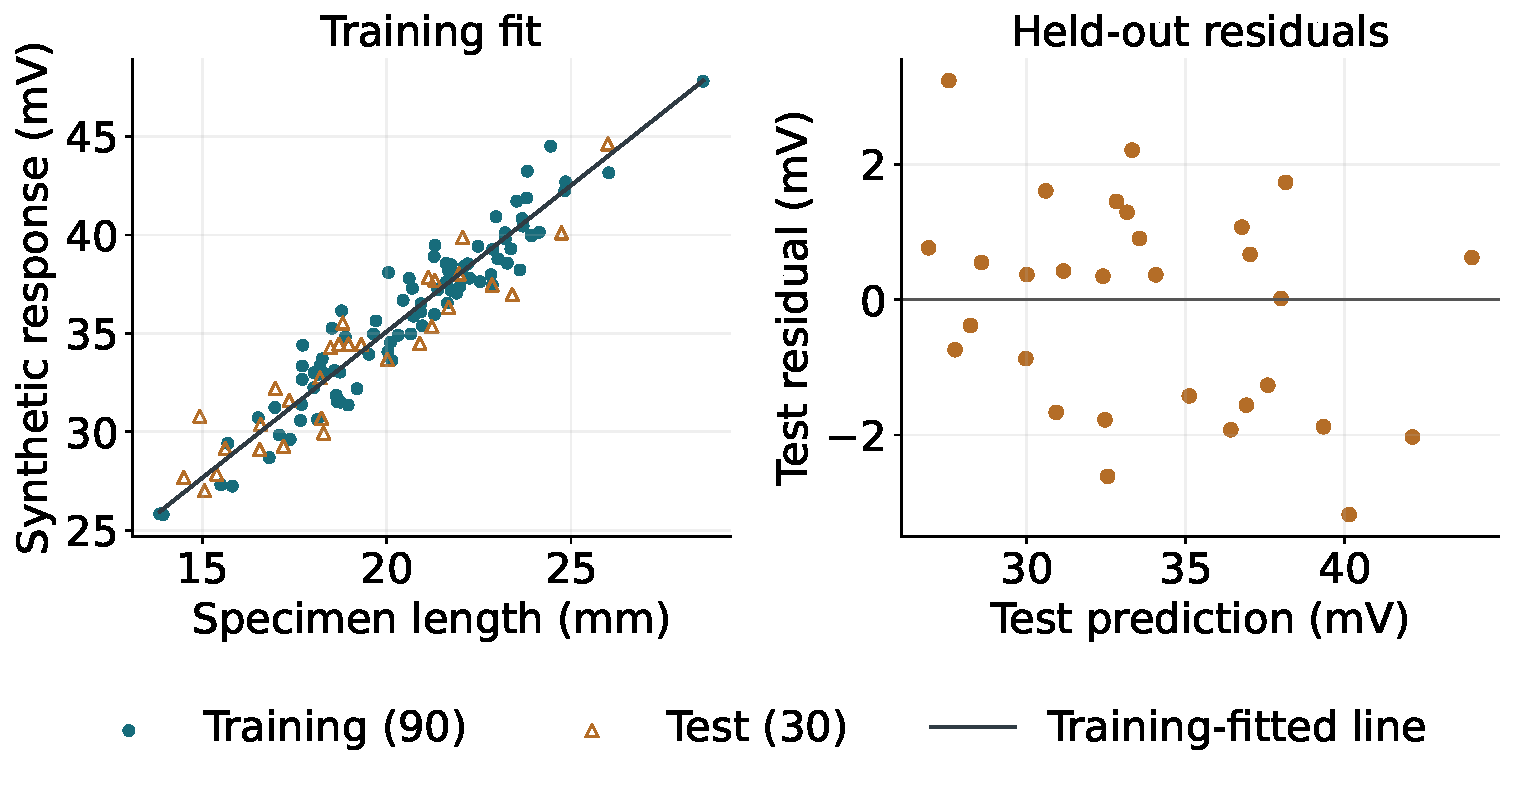
\includegraphics[width=.98\linewidth,height=.69\textheight,keepaspectratio]{regression-and-residuals.pdf}\end{frame}
\renewcommand{\notestarget}{notes.pdf\#note-principal-component-directions}
\begin{frame}[t,fragile,label=slide-projection-and-reconstruction]{Projection and reconstruction}
\[
z=(x-\mu)v_1,\qquad \widehat x=\mu+zv_1^{\mathsf T}.
\]
\pause{}
The reconstruction error is orthogonal to $v_1$. A large retained variance need not preserve information useful for predicting a separate response.
\end{frame}
\renewcommand{\notestarget}{notes.pdf\#note-scaling-and-distance}
\begin{frame}[t,fragile,label=slide-scaling-and-distance]{Scaling and distance}
\[
d^2(x,x')=\sum_j(x_j-x'_j)^2.
\]
\pause{}
\[
z_j=\frac{x_j-\mu_{j,\rm train}}{s_{j,\rm train}},\qquad s_{j,\rm train}>0.
\]
\end{frame}
\renewcommand{\notestarget}{notes.pdf\#note-scaling-and-distance}
\begin{frame}[t,fragile,label=slide-a-zero-variance-coordinate]{A zero-variance coordinate}
If $s_{j,\rm train}=0$, division is undefined.
\pause{}
A fixed rule must remove or separately handle that coordinate. Test data must not determine the training scale.
\end{frame}
\renewcommand{\notestarget}{notes.pdf\#note-the-k-means-objective}
\begin{frame}[t,fragile,label=slide-the-k-means-objective]{The k-means objective}
\[
J(c,\mu)=\sum_i\|x_i-\mu_{c_i}\|_2^2.
\]
\pause{}
\[
c_i=\arg\min_k\|x_i-\mu_k\|_2^2,\qquad
\mu_k=\frac1{|C_k|}\sum_{i\in C_k}x_i.
\] The update requires $|C_k|>0$; empty clusters need a separate rule.
\end{frame}
\renewcommand{\notestarget}{notes.pdf\#note-scaling-and-distance}
\begin{frame}[label=slide-effect-of-feature-units-figure]{Effect of feature units}
\centering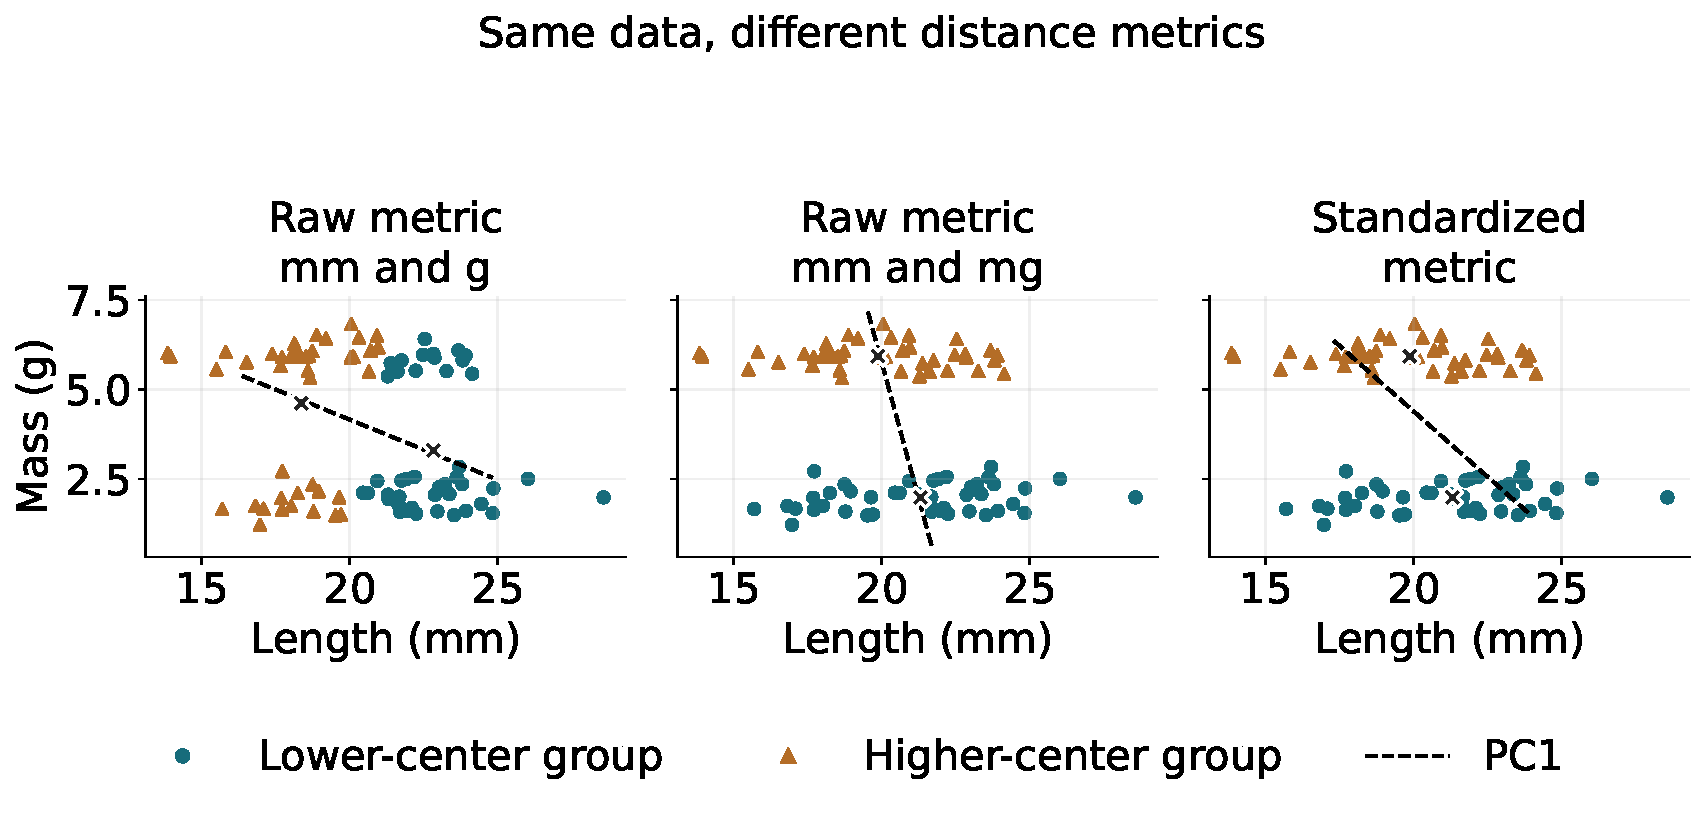
\includegraphics[width=.98\linewidth,height=.69\textheight,keepaspectratio]{scale-projection-groups.pdf}\end{frame}
\renewcommand{\notestarget}{notes.pdf\#note-the-k-means-objective}
\begin{frame}[t,fragile,label=slide-group-labels]{Group labels}
Permuting the center labels leaves the objective unchanged.
\pause{}
Group 0 and group 1 have no intrinsic biological meaning. Interpretation requires information beyond the distance calculation.
\end{frame}
\renewcommand{\notestarget}{notes.pdf\#note-fitted-transformations-and-evaluation}
\begin{frame}[t,fragile,label=slide-fitted-transformations-and-evaluation]{Fitted transformations and evaluation}
\[
\text{training data}\ \longmapsto\ (\mu,s,v_1,\widehat\beta,\widehat\mu_k).
\]
\pause{}
The fitted quantities are then held fixed when transforming and evaluating test observations.
\end{frame}
\renewcommand{\notestarget}{notes.pdf\#note-fitted-transformations-and-evaluation}
\begin{frame}[t,fragile,label=slide-a-numerical-implementation]{A numerical implementation}
\begin{verbatim}
beta = np.linalg.lstsq(A_train, y_train, rcond=None)[0]
y_pred = A_test @ beta
rmse = np.sqrt(np.mean((y_test-y_pred)**2))
\end{verbatim}
No test response enters the coefficient solve.
\end{frame}
\end{document}
